\chapter{Part I: Column Store}
\label{chap:column-store}

In this chapter, we modify how \gap~represents data internally by replacing the original row storage format with a column store. We see how it successfully reduces memory consumption and load times for the \tpchdl. The work undertaken in this chapter lays some important groundwork for further optimization.

This chapter makes up the first out of four main iterations in the design and experiment part of this research. As mentioned in the introduction, we aim to reduce memory consumption in the first iterations of the research. 

\clearpage

\section{Introduction}
\label{sec:Introduction}
% Tell how we want to reduce memory and how database technology comes to the rescue
Starting our main part of the research, we aim to reduce memory footprint in \gap. As we saw in Section \ref{sec:Compression}, lower memory usage are likely to increase performance because most database processes are memory-bound. Moreover, we hypothesize that memory management is expensive and that the number of allocations, as well as the size of the allocated memory chunks, should be reduced. Inspired by the techniques used by read-optimized databases in Chapter \ref{chap:olap} and motivated by the challenges in \gap, we change how data is represented internally within the platform.

% tell why we picked a column store
We choose to implement a column store, which we read about in Section \ref{sec:Column Storage}. The reason for this is two-fold. First, as we saw in the literature study, columns are inherently more compressible. Hence, a column store is better suited to reduce memory consumption and to test our hypothesis about the costs of memory management. Second, the cases where \genus~has experienced performance issues are in situations where a column store is better suited than a row store, for instance the read-intense join and filter operations.

% Tell why we did not pick a row store
We believe that conventional transactional processing in \gap, where a row store might be better suited, will not suffer from using a column store. In \gap, there is much overhead on object create, update, and delete, like constraint checks, data validation, and memory allocations. Thus, we hypothesize that tuple materialization costs and the effects of decreased memory locality are neglible. Also, a row store might require index structures to accommodate certain operations; indexes which, as we have seen in Section \ref{sub:Row Stores vs Column Stores}, are costly to maintain.

\section{Implementation}
\label{sec:Implementation}
In this section, we explain how a column store is implemented in \gap. We change the original row store by introducing data source indexes to \cn{CompositionObject}s and replace \cn{CompositionObjectValueCollection} with a new class we denote as \cn{CompositionValueCollection}.


\subsection{CompositionValueCollection}
\label{sub:CompositionValueCollection}
% Lineout the challenges
As we saw in Section \ref{sec:Challenges in Genus App Platform}, one of the challenges in \gap~is the \cn{CompositionObjectValueCollection} class that has an excessive amount of pointers. Not only does the class hold references to all data for an object, but also pointers to field descriptors. Although this class is self-contained and flexible, there is no need to store the field descriptor references in every row.


To reduce the number of pointers, and to create a column store, we replace instances of \cn{CompositionObjectValueCollection} with a new class which we denote as \cn{CompositionValueCollection}. This class represents the data storage container for objects in a data source. Also, we extend the \cn{CompositionObject} class with a new integer attribute, \vn{DatasourceIndex}, to identify which objects belong to which indexes in the data buffers. The data source index can be thought of a row identifier which we saw in Section \ref{sub:Row Identifiers and Tuple Materialization}.

% Conceptually what is done
\begin{figure}
    \centering
    \begin{subfigure}{1.0\textwidth}
        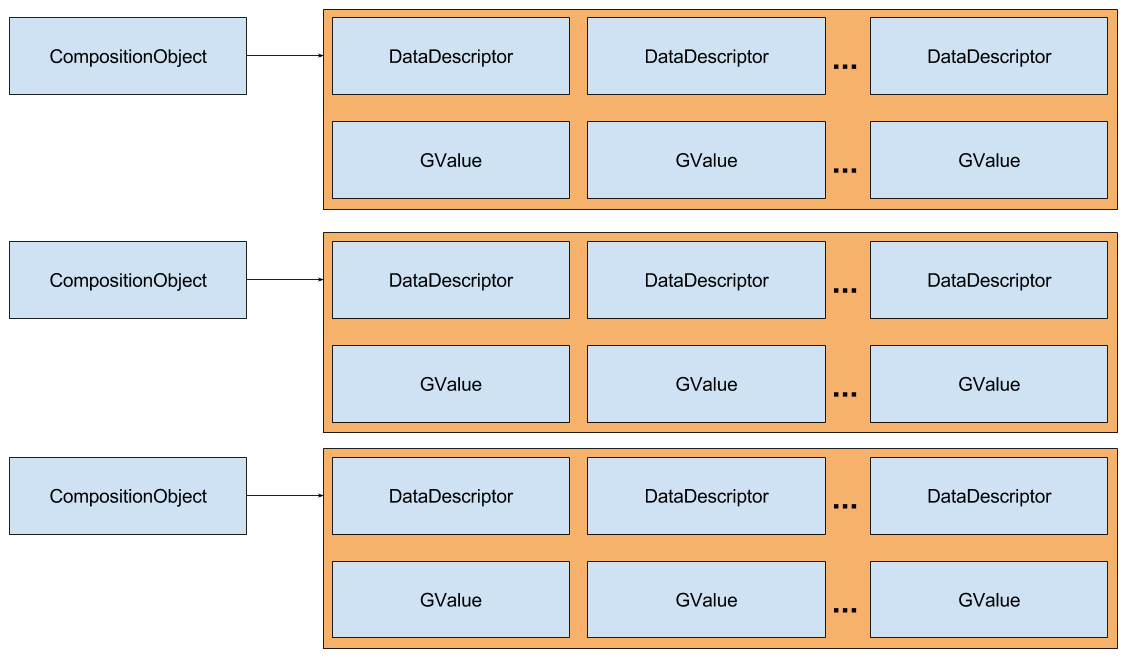
\includegraphics[width=\textwidth]{img/gap-original-rows.png}
        \caption{Original implementation with \cn{CompositionObjectValueCollection}. Each object has its own value collection, and each value collection contains references to both data descriptors and the data itself.}
        \label{fig:gap-original-rows}
    \end{subfigure}
    \begin{subfigure}{1.0\textwidth}
        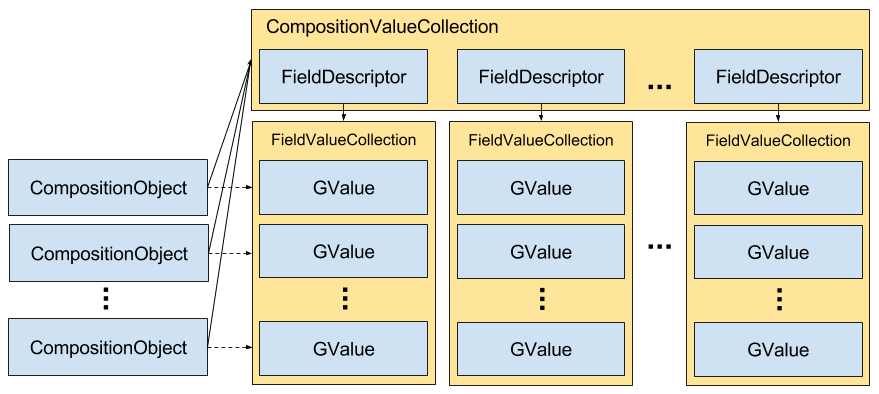
\includegraphics[width=\textwidth]{img/gap-bb-columns.png}
        \caption{Column store implementation with \cn{CompositionValueCollection} and \cn{FieldValueCollection}. All objects in a data source point to the same value collection, and access data using data source indexes and field descriptors to indicate row and column respectively.}
        \label{fig:gap-bb-columns}
    \end{subfigure}
    \caption{Comparison of the original row store implementation in \gap~and the new column store implementation.}
    \label{fig:gap-storage-comparison}
\end{figure}

Our modifications imply that composition objects in a data source no longer queries its own data collection, or \cn{CompositionObjectValueCollection}, for values, but instead request values from one shared \cn{CompositionValueCollection}. To access values in the column store, objects must pass their data source index and a field descriptor to indicate row and column respectively. A comparison between the original and the new implementation is seen in Figure \ref{fig:gap-storage-comparison}. Even though the original \cn{CompositionObjectValueCollection} was discarded as the main data source storage structure, the structure is still in use and can created by the objects. \gap~uses \cn{CompositionObjectValueCollection} extensively in various parts of the application, for instance object cloning and data transfer. \todo{Correct?}


% class diagram
% explain the dictionary and the list of data descriptors
\afigure{img/CompositionValueCollection.png}{\cn{CompositionValueCollection} class diagram.}{fig:CompositionValueCollection}{0.9}
The class diagram for \cn{CompositionValueCollection} is seen in Figure \ref{fig:CompositionValueCollection}. The main methods in this class are \fn{GetValue} and \fn{SetValue}. In these methods, a dictionary lookup finds the correct column, or \cn{FieldValueCollection}, and requests the value for the given data source index. \cn{IsAssigned} and \cn{UnassignValue} work similarly. In addition to the access methods for single data elements, row- or column-wise operations like \fn{UnassignAllValues} exist. 

Data source indexes are assigned by passing composition objects to the \fn{RegisterObject} method. A private variable, \vn{maxDatasourceIndex} is used to keep track of the maximum index assigned so far. When an object is removed from a data source, \cn{RemoveObject} is called, and this method keeps track of removed objects in the \vn{assignedIndexes} bitmap.

%The \fn{Consolidate} function is called by the data source when it is done loading and is meant to be an operation where the column store restructures and maximizes space utilization. We see how the columns are affected by this operation in the section about growth strategy, Section \ref{sec:Growth Strategy}.

%The main methods in the \cn{CompositionValueCollection} class is the \fn{setValue} and \fn{getValue} methods. These functions respectivel set and get \cn{GValues} for a data descriptor and a datasource index. In these operations, the correct column, or \cn{FieldValueCollection}, is looked up in a dictionary, and the index is passed along to the column to get or set the value. If no column exist for a data descriptor, it is created. \fn{isAssigned} and \fn{unassignValue} works similarly. We study the unassigned semantic in Section \ref{sub:Unassigned Values}. 

%Datasource indexes are assigned by passing composition objects to the  \fn{registerObject} function. A private variable \vn{maxDatasourceIndex} is used to keep track on the maximum index handed out so far. When an object is received, this variable is incremented, and the object is assigned that value. In addition to this, a bitmap \fn{assignedIndexes} is kept to bookkeep which indexes has objects connected to them. When \fn{removeObject} is called, the bit for that index is unset in \fn{assignedIndexes}. Also, all values corresponding to that object are unassigned. Currently, the \fn{assignedIndexes} bitmap is not used to lookup the first available bit, since this triggers a linear search on every insertion. We discuss this further in the chapter conclusion.

%In addition to the above methods, a \cn{CompositionValueCollection} has the ability to unassign an entire row or column by passing in a \cn{CompositionObject} or \cn{DataDescriptor} respectively. We see later in this research where such methods are used.



\subsection{FieldValueCollection}
\label{sub:FieldValueCollection}
\afigure{img/FieldValueCollection.png}{\cn{FieldValueCollection} class diagram.}{fig:FieldValueCollection}{0.55}

We implement columns as a class we denote as \cn{FieldValueCollection}. This class represents an index based list structure that automatically handles memory allocation. Internally, values are stored in a \cn{TArray<GValue>} type. We chose that structure based on the performance benchmark in Appendix \ref{app:array-performance}. A class diagram is found in Figure \ref{fig:FieldValueCollection}. 

Besides from the value array and corresponding \fn{GetValue} and \fn{SetValue} methods, \cn{FieldValueCollection} contains bitmaps for indicating null values and unassigned values. Keeping track of null values is strictly not needed, since \cn{GValue}s are boxed and can be set to \nil, but it becomes appearent why we need this bookkeeping in Chapter \ref{chap:storage-format}. Unassigned values have a special semantic in \gap: It means that a value exist, but has been unassigned for performance reasons. 

\subsection{Growth Strategy}
\label{sub:Growth Strategy}

In \cn{FieldValueCollection} we use \delphi~dynamic arrays for data and are, therefore, in control over array allocation size. Since objects arrive in a data stream, we are not sure how large our buffers should be until we receive all objects. Hence, we must find an efficient growth strategy for the column store.

For every array resize, we run the risk that all data in the array must be copied from one smaller memory chunk to a larger one. Since this is a costly operation, one should be generous when resizing arrays. Commonly used in such problems is a doubling strategy, where array buffer size double each time an index outside of array bounds appear. We implement this behaviour in \cn{CompositionValueCollection} too, in the \fn{EnsureCapacity} method. This function is called to avoid index-out-of-range exceptions by all methods that access the data array or bitmaps.

\afigure{img/gap-growth-strategy.png}{Growth strategy for value buffers and bitmaps. In the load phase, the buffers double every time more space is needed. After the load phase, a consolidation is performed which reduces buffer size to the exact size of the data source.}{fig:gap-growth-strategy}{0.6}
Using the doubling strategy for column growth, we run the risk of allocating twice as much memory needed for a data source. We, therefore, implement a \cn{Consolidate} method which resizes all value buffers and bitmaps to the exact size of the data source. The full growth strategy in depicted in Figure \ref{fig:gap-growth-strategy}

In \cn{CompositionValueCollection}, columns are created on-demand as composition objects set values. If an object requests a value from a column that does not exist, \nil~is returned.

\subsection{CompositionObject Modification}
\label{sub:CompositionObject Modification}
To accommodate the new \cn{CompositionValueCollection} class, we perform some modifications to the \cn{CompositionObject} class. First and foremost, we replace the \cn{CompositionObjectValueCollection} member variable with a pointer to the column store. At the same time, we remove all code that accesses the original row structure and replace it with calls to the \cn{CompositionValueCollection} instance. For all interaction with this class, the data source index is passed to indicate which row the composition object belongs. Second, we call \fn{RegisterObject} within the constructor of the \cn{CompositionObject} class, such that a data source index is assigned. Analogously, \fn{RemoveObject} is called in the destructor.

Some methods in \cn{CompositionObject} require a new implementation as a result of the column store. These methods include \fn{CloneValueCollectcion} and \fn{AdoptValueCollection}. Earlier, these methods were trivial, as they only cloned and replaced \cn{CompositionObjectValueCollection} instances. However, since composition objects no longer have ownership in such structures, they must be cloned or adapted by iterating field descriptors and reading or writing data in the column store.

\section{Results}
\label{sec:Results}
We test the changes done in this iteration by using Benchmark \ref{bm:q1}, the \tpchdl. We use this benchmark to see whether memory footprint has been reduced. We are also curious to see the performance impact on data load time, lookup index generation (join), and source measure lookup. To see whether our changes has caused negative effects on write performance, we also run Benchmark \ref{bm:write}, the \textit{Write Benchmark}. Full benchmark details are found in Appendix \ref{app:bm}.

In this iteration, we test two different configurations: The original \gap~implementation and the new column store. Due to time constraints, we run our benchmarks only three times and report the mean. All measurements had low variance, within 15 \% of the average measurement.

\subsection{Data Mart Load Benchmark}
\label{column-store:q1}

\afigure{img/column-store-bpl.png}{Bytes per \lineitem~used by the original and column store impelementations, Benchmark \ref{bm:q1} with scaling factors SF0.01 and SF0.1.}{fig:column-store-bpl}{0.9}
In the \tpchdl, we found a significant memory reduction in the column store implementation. As we see in Figure \ref{fig:column-store-bpl}, for SF0.01 the memory used per \lineitem~is reduced with 38 \%, and for SF0.1 the reduction is 30 \%. The total application memory footprint for the analysis is reduced from 2685 MB to 1777 MB.

\begin{figure}
    \centering
    \begin{subfigure}{0.7\textwidth}
        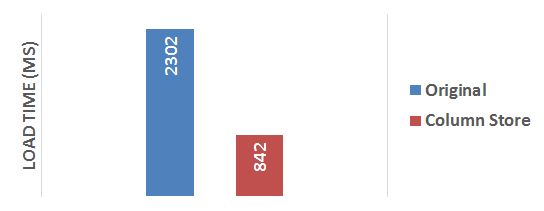
\includegraphics[width=\textwidth]{img/column-store-load-sf001.png}
        \caption{SF0.01}
    \end{subfigure}
    \begin{subfigure}{0.7\textwidth}
        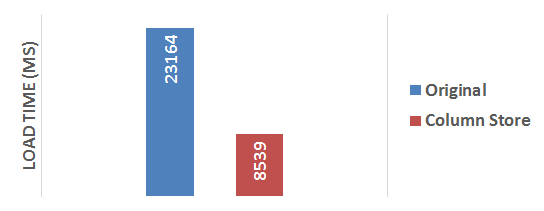
\includegraphics[width=\textwidth]{img/column-store-load-sf010.png}
        \caption{SF0.1}
    \end{subfigure}
    \caption{Data source load time for for original and column store implementations, Benchmark \ref{bm:q1} with scaling factors SF0.01 and SF0.1.}
    \label{fig:column-store-load}
\end{figure}
In Figure \ref{fig:column-store-load}, we see that the load time also is significantly reduced using the new \cn{CompositionValueCollection} class. For both scaling factors, the time it takes to populate the data source has been reduced by 63 \%. 


\begin{figure}
    \centering
    \begin{subfigure}{0.9\textwidth}
        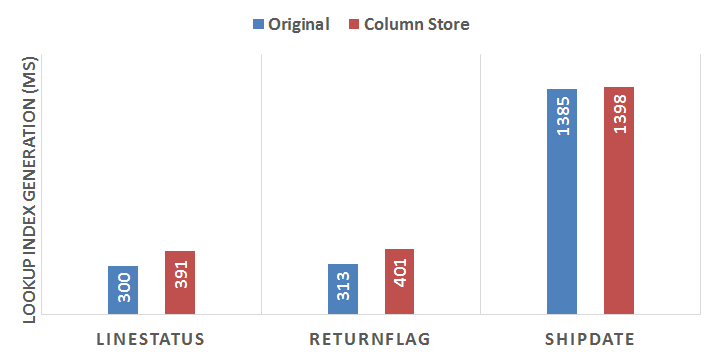
\includegraphics[width=\textwidth]{img/column-store-lig-sf001.png}
        \caption{SF0.01}
    \end{subfigure}
    \begin{subfigure}{0.9\textwidth}
        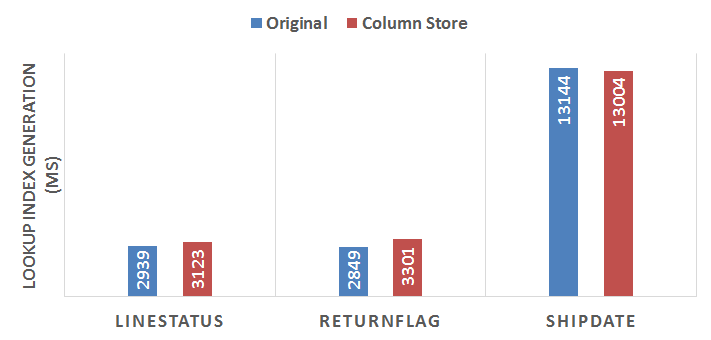
\includegraphics[width=\textwidth]{img/column-store-lig.png}
        \caption{SF0.1}
    \end{subfigure}
    \caption{Lookup index generation performance comparison for \texttt{LINESTATUS}, \texttt{RETURNFLAG}, and \texttt{SHIPDATE}, Benchmark \ref{bm:q1} with scaling factors SF0.01 and SF0.1.}
    \label{fig:column-store-lig}
\end{figure}
We observe that lookup index generation, or the join operation, is slightly hurt performance-wise by the \cn{CompositionValueCollection} implementation. For SF0.01, the time it takes to perform a join between \texttt{RETURNFLAG} and \texttt{LINEITEM} tables is increased by approximately 30 \%. We measure similar changes for SF0.1, but the percentage difference is smaller.

\begin{figure}
    \centering
    \begin{subfigure}{1.0\textwidth}
        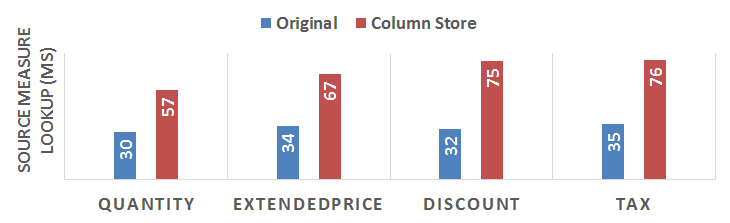
\includegraphics[width=\textwidth]{img/column-store-sml-sf001.png}
        \caption{SF0.01}
    \end{subfigure}
    \begin{subfigure}{1.0\textwidth}
        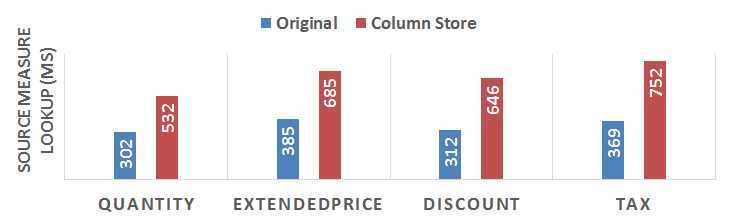
\includegraphics[width=\textwidth]{img/column-store-sml-sf010.png}
        \caption{SF0.1}
    \end{subfigure}
    \caption{Source measure lookup operation performance comparison for \texttt{QUANTITY}, \texttt{EXTENDEDPRICE}, \texttt{DISCOUNT}, and \texttt{TAX}, Benchmark \ref{bm:q1} with scaling factors SF0.01 and SF0.1.}
    \label{fig:column-store-sml}
\end{figure}

We observe a larger reduction in performance looking at the source measure lookup operation in Figure \ref{fig:column-store-sml}. Here, the time it takes to extract all values in a column into a floating point number array is doubled. We measure the same effect for both scaling factors.

\subsection{Write Benchmark}
\label{sub:Write Benchmark}
\afigure{img/column-store-write.png}{Write performance results for Benchmark \ref{bm:write}, 1000 elements..}{fig:column-store-write}{1.0}
To see how the write speed is affected by our new implementation, we run Benchmark \ref{bm:write}, the \textit{Write Benchmark} on the original implementation and the column store implementation. Each run modified 1000 elements, which is the default for this benchmark. The results are presented in Figure \ref{fig:column-store-write}. There are no significant differences between the two implementations.

\section{Discussion}
\label{sec:Discussion}
% How it impacts memory
In Section \ref{sub:Excessive Amount of Pointers}, we saw how a data source with objects with 15 properties each needed 32 pointers, or 256 bytes, per objects just for data and data access. Now, this number is reduced to 17 pointers and an integer, which is 140 bytes. Hence, we have the potential to save 45\% memory by using our new system.

We see that the memory used per object in the \tpchdl~is reduced by 30 \% and 38 \% for scaling factors 0.1 and 0.01 respectively. We attribute this observation to the column store, and how it reduces the number of pointers needed to represent data in a data source. 

We are observe that the data source load time is reduced as a consequence of our new \cn{CompositionValueCollection} and \cn{FieldValueCollection} classes. This observation strengthens our hypothesis that memory management is expensive: The original implementation allocated one row-structure per object, whereas the doubling strategy in our column store keeps the number of allocations at a minimum. Moreover, the reduced load time in Benchmark \ref{bm:q1}~might also imply that reduced memory usage is directly correlated with performance and that our new implementation has better memory locality and cache hit rate.

Both read operations, lookup index generation and source measure lookup, suffer from the new column store implementation. On these operations, the time it takes to perform the operation has been increased by 30 \% and 100 \% respectively. Since both operations read values intensively from composition objects in tight loops, we believe the test result implies that the \fn{GetValue} function in the column store is not as efficient as the original. This can be caused by the dictionary lookup to find the correct column, or by the extra checks to ensure capacity or for \nil~values.

The fact that Benchmark \ref{bm:write}, the \textit{Write Benchmark}, shows that write performance is not affected by the column store, strengthens our hypothesis that the column overhead is negligible in such situations. Data modification is expensive in \gap. Modifying 1000 elements in the write benchmark takes roughly five times longer than generating a lookup index for 60,000 rows, which indicates that there is a severe overhead in object iteration and value modification unrelated to the data storage layout.

We are unsure why different scaling factors yielded a different number of bytes per \lineitem. It might be caused by the caching and value reuse mechanisms used by the data load module in \gap. Data in SF0.1 might have a different data distribution than SF0.01. Either way, both the original and column store implementations are affected by this phenomenon, which makes it likely that it is unrelated to our work. The other measurements in \tpchdl~increase linearly, measurements from SF0.1 are roughly ten times higher than for SF00.1. 

\section{Iteration Conclusion}
\label{sec:Iteration Conclusion}
We conclude this iteration by stating that there is a large potential in column storage regarding memory footprint and load times. Memory used per \lineitem~in the \tpchdl~has been reduced by 30 - 38 \%, and the time it takes to load all data in this benchmark by 67 \%. Write performance, tested with Benchmark \ref{bm:write}, has not been affected by the new implementation.

Still, both read-intense operations tested in Benchmark \ref{bm:q1} are slowed down, especially the source measure lookup operation. Here, the time it takes to generate an array of double precision numbers for a data descriptor is doubled with the column store. We believe these changes are caused by a \fn{GetValue} function less efficient than the original.

This iteration lays the groundwork for further investigation and to check whether database technologies and column store can help \mdd-tools' ability to handle and analyze large datasets. We believe even more memory can be saved by optimizing storage formats, applying compression, and removing more pointers. We do this in the next iterations, Chapter \ref{chap:storage-format} and Chapter \ref{chap:compression}. 

Column storage comes with several benefits, like vectorized execution, late materialization, and the ability to be pipelined by a modern CPU. We have not yet utilized the full potential of the \cn{CompositionValueCollection} and \cn{FieldValueCollection} classes, so far we have only used them to reduce the number of pointers in \gap. We believe the mentioned techniques can be applied to the read-intense operations of Benchmark \ref{bm:q1}. We study this in Chapter \ref{chap:operations}.

Since the measurements for different scaling factors in the \tpchdl~increase linearly, that is, measurements from SF0.1 are roughly ten times higher than for SF0.01; we will focus on SF0.1 from now. For the next iterations, we run tests with both SF0.01 and SF0.1, but we generally only report and discuss the results from SF0.1. An exception to this is the number of bytes per \lineitem, where we continue to report on both scaling factors.

\subsection{Future Work}
\label{sub:column-store:future-work}
With our current solution, new data source indexes, or row identifiers, are assigned by incrementing a counter in \cn{CompositionValueCollection}. This implies that if objects are removed from a data source, no new objects will be assigned the data source indexes that has become available. As seen in Figure \ref{fig:CompositionValueCollection}, we propose a \textit{bitmap for assigned indexes}, \vn{assignedFlags}. Future work might investigate the effects of using this bitmap, and the \fn{OpenBit} utility function, to assign indexes to a data source. Since \fn{OpenBit} is a linear-time operation, one might consider an object loading state: Indexes are assigned by using a counter if the data source is fed with data from the database, and once this operation has completed, the \vn{assignedFlags} bitmap is used.

In Section \ref{sub:Horizontal Partitioning}, we saw that horizontal partitioning of columns may be beneficial for a column store for several reasons, like metadata pruning, handling of data skew, and parallelism. By introducing a \vn{PartitionIndex} variable in addition to \vn{DatasourceIndex}, and change the column store interface to accommodate the new index, horizontal partitioning can be made possible in \gap. Future work should elaborate on the changes needed in \cn{CompositionValueCollection} and \cn{FieldValueCollection} to enable horizontal partitioning, and investigate the effects of this technique.

%In addition, we have observed that the bytes per \texttt{LINEITEM} is increased on larger data sets, and we believe this is caused by the caching and value reuse mechanisms in the data source loader. However, larger datasets should be able to reuse more values, not less. We therefore encourage studying this peculiar effect in future work.

%\begin{table}
%    \centering
%    \begin{tabularx}{0.9\textwidth}{X | X X X}
%        SF0.01 & \texttt{LINESTATUS} & \texttt{RETURNFLAG} & \texttt{SHIPDATE}\\ 
%        \hline
%        \hline
%        Original & 300 ms & 313 ms & 1385 ms \\
%        Column Store & 391 ms & 401 ms & 1398 ms \\
%    \end{tabularx}
%    \newline
%    \vspace*{1 cm}
%    \newline
%    \begin{tabularx}{0.9\textwidth}{X | X X X}
%        SF0.1 & \texttt{LINESTATUS} & \texttt{RETURNFLAG} & \texttt{SHIPDATE}\\ 
%        \hline
%        \hline
%        Original & 2939 ms & 2849 ms & 13144 ms \\
%        Column Store & 3123 ms & 3301 ms & 13004 ms \\
%    \end{tabularx}
%    \caption{Lookup index generation performance comparison for \texttt{LINESTATUS}, \texttt{RETURNFLAG}, and \texttt{SHIPDATE} for SF0.01 (upper) and SF0.1 (lower).} 
%    \label{tab:non-blackbox-lig}
%\end{table}

%For the \tpchdl, we used both scaling factors, SF0.01 and SF0.1.
%\begin{table}
%    \centering
%    \begin{tabularx}{0.75\textwidth}{X | X X}
%        & SF0.01 & SF0.1 \\ 
%        \hline
%        \hline
%        Original & 674 bytes & 715 bytes \\
%        Column Store & 419 bytes & 501 bytes \\
%        \% reduction & 38 \% & 30 \% \\
%    \end{tabularx}
%    \caption{Bytes per \texttt{LINEITEM} used by the original and the new column store implementation.} 
%    \label{tab:non-blackbox-bpl}
%\end{table}

%\begin{table}
%    \centering
%    \begin{tabularx}{0.75\textwidth}{X | X X}
%        & SF0.01 & SF0.1 \\ 
%        \hline
%        \hline
%        Original & 2302 ms & 23164 ms \\
%        Column Store & 842 ms & 8539 ms \\
%        \% reduction & 63 \% & 63 \% \\
%    \end{tabularx}
%    \caption{Load times for Benchamrk \ref{bm:q1} for the original and the new column store implementation and scaling factors 0.01 and 0.1.} 
%    \label{tab:non-blackbox-load}
%\end{table}

%\begin{table}
%    \centering
%    \begin{tabularx}{\textwidth}{X | X X X X}
%        SF0.01 & \texttt{QUANTITY} & \texttt{EXTENDEDPRICE} & \texttt{DISCOUNT} & \texttt{TAX}\\ 
%        \hline
%        \hline
%        Original & 30 ms & 34 ms & 32 ms & 35 ms \\
%        Column Store & 57 ms & 67 ms & 75 ms & 76 ms
%    \end{tabularx}
%    \newline
%    \vspace*{1 cm}
%    \newline
%    \begin{tabularx}{\textwidth}{X | X X X X}
%        SF0.01 & \texttt{QUANTITY} & \texttt{EXTENDEDPRICE} & \texttt{DISCOUNT} & \texttt{TAX}\\ 
%        \hline
%        \hline
%        Original & 302 ms & 385 ms & 312 ms & 369 ms \\
%        Column Store & 532 ms & 625 ms & 646 ms & 752 ms
%    \end{tabularx}
%    \caption{Source measure lookup for \texttt{QUANTITY} \texttt{EXTENDEDPRICE}, \texttt{DISCOUNT}, and \texttt{TAX} for SF0.01 (upper) and SF0.1 (lower).} 
%    \label{tab:non-blackbox-sml}
%\end{table}
